\begin{frame}
\begin{columns}[c]
\column{.5\textwidth}

\psset{xunit=0.7cm, yunit=0.7cm}
\begin{pspicture}(-2.6, -2.5)(4.1,2.6)
\psframe*[linecolor=white](-2.6,-2.5)(4.1,2.6)
\tiny
\fcAxesStandard{-2.6}{-2.5}{5}{2.6}
\fcLabelXOne
\uncover<2>{
\psline[linecolor=red](-2.5, -1.5)(1.5, 2.5)
}
\uncover<3->{
\psline[linecolor=blue](-2.5, -1.5)(1.5, 2.5)
}
\uncover<2->{
\rput[l](1.5, 2){$y=x+1$}
}
\uncover<5->{
\fcFullDot{0}{1}
\rput[r](-0.1, 1){\alert<5>{$(0,1)$}}
}

\uncover<3>{
\psline[linecolor=red](-2.5, 1.25)(5, -2.5)
}
\uncover<4->{
\psline[linecolor=blue](-2.5, 1.25)(5, -2.5)
}
\uncover<3->{
\rput[r](3.3, -2){$y=-0.5x$}
}
\uncover<6->{
\fcFullDot{0}{0}
\rput[lb](0.1, 0.1){\alert<6>{$(0,0)$}}
}

\uncover<4>{
\psline[linecolor=red](-2.5,-1)(5, -1)
}
\uncover<5->{
\psline[linecolor=blue](-2.5, -1)(5, -1)
}
\uncover<4->{
\rput[t](4, -1.1){$y=-1$}
}
\uncover<7->{
\fcFullDot{0}{-1}
\rput[lt](0.1, -1.1){\alert<7>{$(0,-1)$}}
}
\end{pspicture}
%\ \only<handout:0| -2>{%
%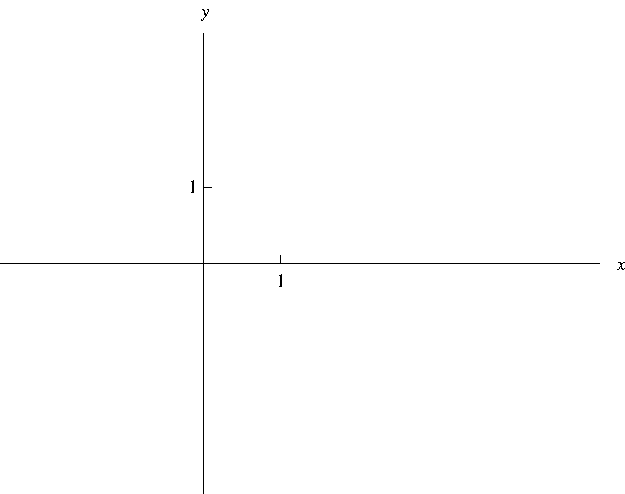
\includegraphics[height=4.5cm]{precalculus/pictures/01-02-linesa.pdf}%
%}%
%\only<handout:0| 3>{%
%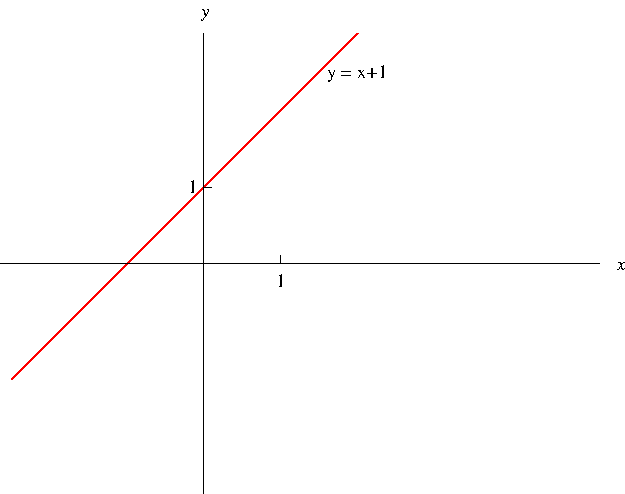
\includegraphics[height=4.5cm]{precalculus/pictures/01-02-linesb.pdf}%
%}%
%\only<handout:0| 4>{%
%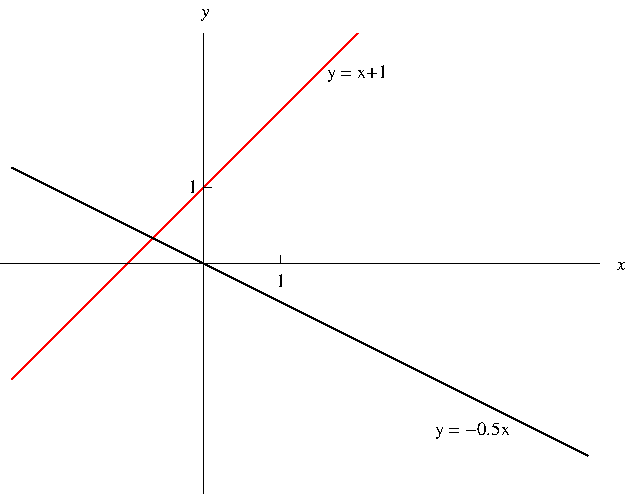
\includegraphics[height=4.5cm]{precalculus/pictures/01-02-linesc.pdf}%
%}%
%\only<handout:0| 5>{%
%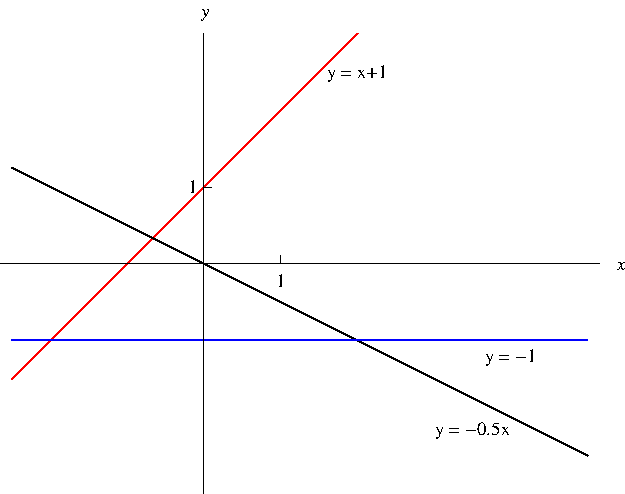
\includegraphics[height=4.5cm]{precalculus/pictures/01-02-linesd.pdf}%
%}%
%\only<handout:0| 6>{%
%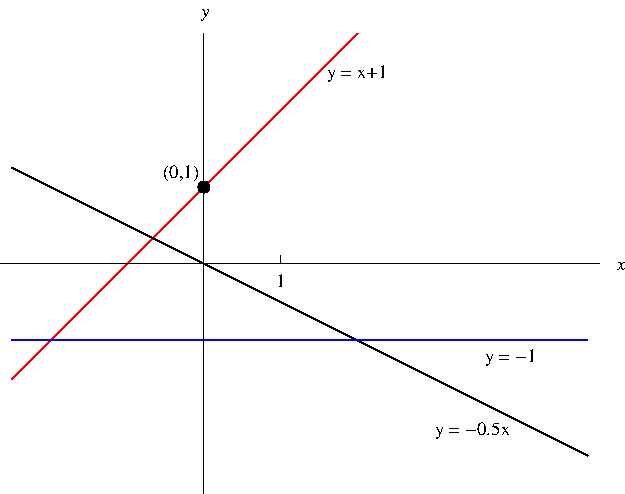
\includegraphics[height=4.5cm]{precalculus/pictures/01-02-linese.pdf}%
%}%
%\only<handout:0| 7>{%
%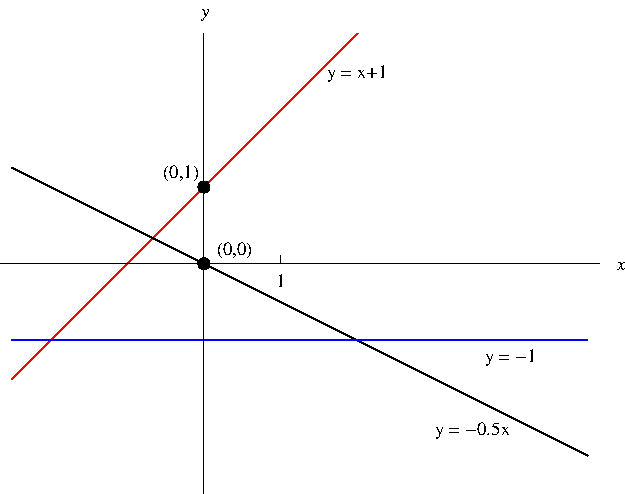
\includegraphics[height=4.5cm]{precalculus/pictures/01-02-linesf.pdf}%
%}%
%\only<8>{%
%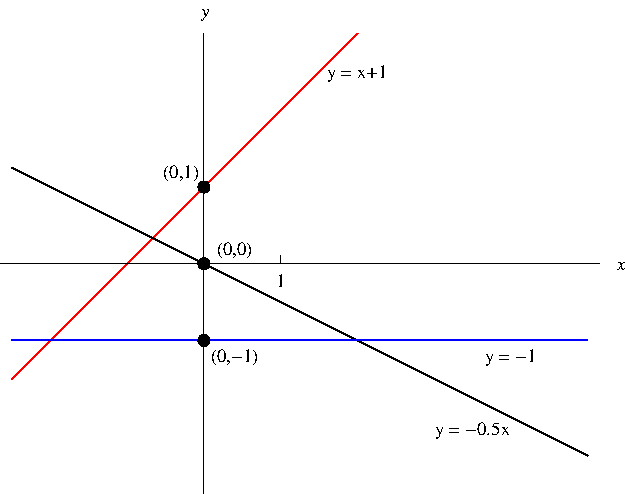
\includegraphics[height=4.5cm]{precalculus/pictures/01-02-linesg.pdf}%
%}%
\column[t]{.55\textwidth}
\begin{tabular}{|c|c|c|}
\hline
$f(x)$ & Direction & $y$-intercept \\
\hline
\uncover<1->{\alertNoH{ 2}{$x + \alertNoH{ 5}{1}$}} &
\uncover<2->{\alertNoH{ 2}{$\nearrow$}} &
\uncover<5->{\alertNoH{ 5}{1}} \\
\uncover<1->{\alertNoH{ 3}{$-0.5x \uncover<6>{\alertNoH{ 6}{+ 0}}$}} &
\uncover<3->{\alertNoH{ 3}{$\searrow$}} &
\uncover<6->{\alertNoH{ 6}{0}} \\
\uncover<1->{\alertNoH{ 4,7}{$-1$}} &
\uncover<4->{\alertNoH{ 4}{$\rightarrow$}} &
\uncover<7->{\alertNoH{ 7}{-1}} \\
\hline
\end{tabular}
\end{columns}

\begin{itemize}
\item<2->  $m > 0$ means the graph of $f$ points up ($\nearrow$).
\item<3->  $m < 0$ means the graph of $f$ points down ($\searrow$).
\item<4->  $m = 0$ means the graph of $f$ is horizontal ($\rightarrow$).
\item<5->  $b$ tells us the height of the point where the graph hits the $y$-axis.
\end{itemize}
\end{frame}